% Overleaf: Menu → Compiler → LuaLaTeX に設定してください
\documentclass[aspectratio=169, 11pt]{beamer}

% ===== Metropolis Theme =====
\usetheme[progressbar=frametitle, numbering=fraction, block=fill]{metropolis}

% ===== Compress Metropolis spacing =====
\makeatletter
\setlength{\metropolis@frametitle@padding}{1.5ex}
\makeatother
\setlength{\leftmargini}{1em}

% ===== Japanese support =====
\usepackage{luatexja}
\usepackage[haranoaji]{luatexja-preset}

% ===== Packages =====
\usepackage{amsmath, amssymb, mathtools}
\usepackage{physics}
\usepackage{tikz}
\usetikzlibrary{arrows.meta, decorations.pathmorphing, patterns}
\usepackage{xcolor}
\usepackage{booktabs}
\usepackage{graphicx}
\usepackage{siunitx}
\usepackage{appendixnumberbeamer}
% Compress Beamer list spacing (enumitem conflicts with Beamer)
\setbeamertemplate{itemize/enumerate body begin}{\vspace{-0.3em}}
\setbeamertemplate{itemize/enumerate body end}{\vspace{-0.2em}}

% ===== Custom colors =====
\definecolor{accent}{RGB}{230,126,34}
\definecolor{darkblue}{RGB}{23,67,88}
\definecolor{alertred}{RGB}{192,57,43}

\setbeamercolor{frametitle}{bg=darkblue}
\setbeamercolor{progress bar}{fg=accent}
\setbeamercolor{alerted text}{fg=alertred}

% ===== Custom commands =====
\newcommand{\highlight}[1]{\colorbox{yellow!30}{$\displaystyle #1$}}
\newcommand{\importantbox}[1]{%
  \begin{center}
  \fcolorbox{darkblue}{blue!5}{\parbox{0.75\textwidth}{\centering\small #1}}
  \end{center}
}
\newcommand{\teacher}[1]{{\color{darkblue}\textbf{→ #1}}}

% ===== Title =====
\title{物理化学 6}
\subtitle{量子化学の基礎}
\author{大学院入試 備考資料}
\date{}
\institute{化学システム工学専攻}

\begin{document}

\maketitle

% ============================================================
\begin{frame}{この講義の目標}

量子化学は「式が多くて難しそう」と思われがちですが，\\
実は\alert{たった一つの方程式}を解くだけの話です。

\vspace{0.3em}
\importantbox{
  Schrödinger方程式 $\hat{H}\psi = E\psi$ を具体的な$V(x)$のもとで解く → エネルギーと波動関数が分かる
}

\textbf{今日の流れ：}
\begin{enumerate}
  \item なぜ古典力学ではダメなのか？
  \item Schrödinger方程式の導出
  \item 変数分離法 → 井戸型ポテンシャル
  \item 物理的意味と応用（共役ポリエン）
  \item 分子振動（調和振動子・Morse）
  \item 黒体放射の定量（Wien則・Stefan-Boltzmann則）
\end{enumerate}
\end{frame}

% ============================================================
\begin{frame}{目 次}
\tableofcontents
\end{frame}

% %%%%%%%%%%%%%%%%%%%%%%%%%%%%%%%%%%%%%%%%%%%%%%%%%%%%%%%%%%%%
\section{なぜ古典力学ではダメなのか}
% %%%%%%%%%%%%%%%%%%%%%%%%%%%%%%%%%%%%%%%%%%%%%%%%%%%%%%%%%%%%

% ============================================================
\begin{frame}{古典論の破綻：黒体放射}

まず，量子論がなぜ必要になったかを見ましょう。

\begin{columns}[c]
\begin{column}{0.55\textwidth}
高温の物体は光を放ちます（\textbf{黒体放射}）。\\
古典論で計算すると：

\[
  \rho(\lambda, T) = \frac{8\pi k_\mathrm{B} T}{\lambda^4}
\]

{\small（$\rho$：エネルギースペクトル密度，$\lambda$：波長，$k_\mathrm{B}$：ボルツマン定数）}

\vspace{0.3em}
\teacher{$\lambda \to 0$（短波長）で$\rho \to \infty$に発散}

これは実験と全く合わない。\\
この矛盾を\alert{紫外破綻}（UV catastrophe）と呼びます。
\end{column}
\begin{column}{0.45\textwidth}
  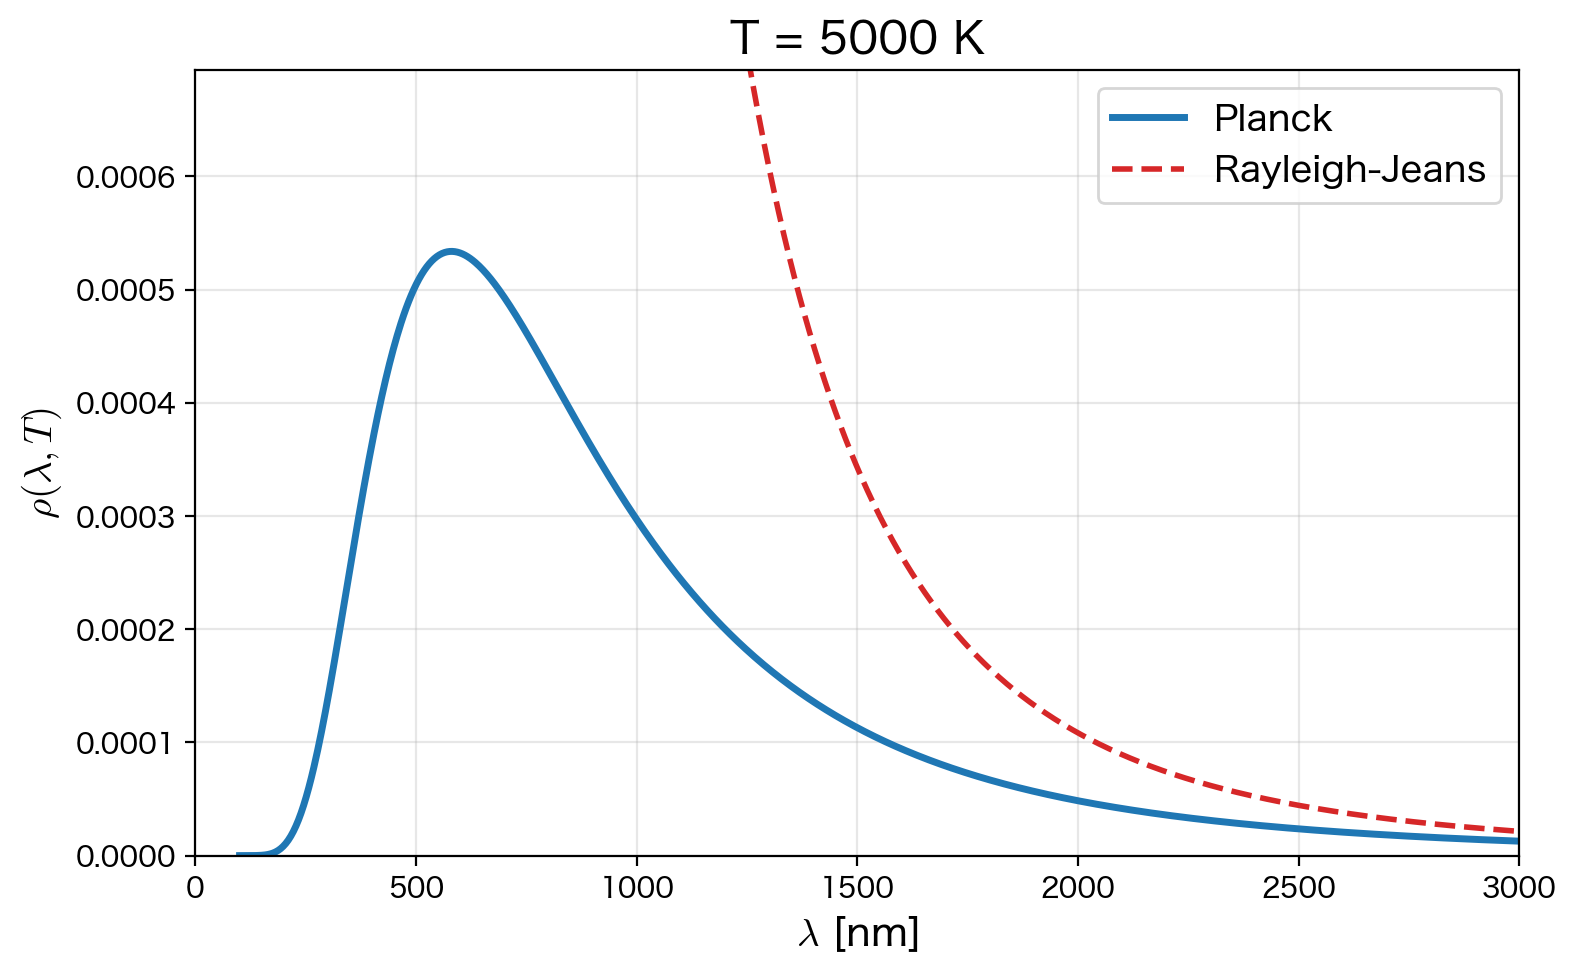
\includegraphics[width=\textwidth]{figures/blackbody.png}
\end{column}
\end{columns}

\end{frame}

% ============================================================
\begin{frame}{Planckの革命的アイデア}

\textbf{Planck (1900)} はこの矛盾を解決するために，\\
古典論の常識を捨てて，大胆な仮定を置きました：

\vspace{0.6em}
\importantbox{
  \textbf{Planckの量子仮説：}\\[4pt]
  電磁波のエネルギーは連続的ではなく，\\
  $h\nu$（$h$：Planck定数，$\nu$：振動数）の\alert{整数倍}でしか取れない。
  \[
    E = nh\nu \qquad (n = 1, 2, 3, \ldots)
  \]
}

\vspace{0.3em}
$h = \SI{6.626e-34}{J.s}$（Planck定数）：とてつもなく小さい値

\vspace{0.3em}
\teacher{日常のスケールでは$h$が小さすぎて量子化に気づかない。\\
原子・分子のスケールで初めて効いてくる。}
\end{frame}

% ============================================================
\begin{frame}{光電効果：光は粒子でもある}

次に，\textbf{Einstein (1905)} がPlanckのアイデアをさらに推し進めました。

\begin{columns}[c]
\begin{column}{0.55\textwidth}
金属に光を当てると電子が飛び出す（\textbf{光電効果}）。

\vspace{0.3em}
\textbf{古典論の予測：}光を強くすれば電子は出るはず\\
\textbf{実験事実：}光の振動数$\nu$が閾値以下なら，\\
\hspace{3em}どんなに強くしても電子は\alert{出ない}

\vspace{0.3em}
\teacher{Einsteinの説明：光は$h\nu$のエネルギーを持つ粒（\textbf{光子}）である。}

\[
  E_\text{kinetic} = h\nu - W
\]
{\small $W$：仕事関数（金属から電子を引き離すのに必要なエネルギー）}
\end{column}
\begin{column}{0.45\textwidth}
  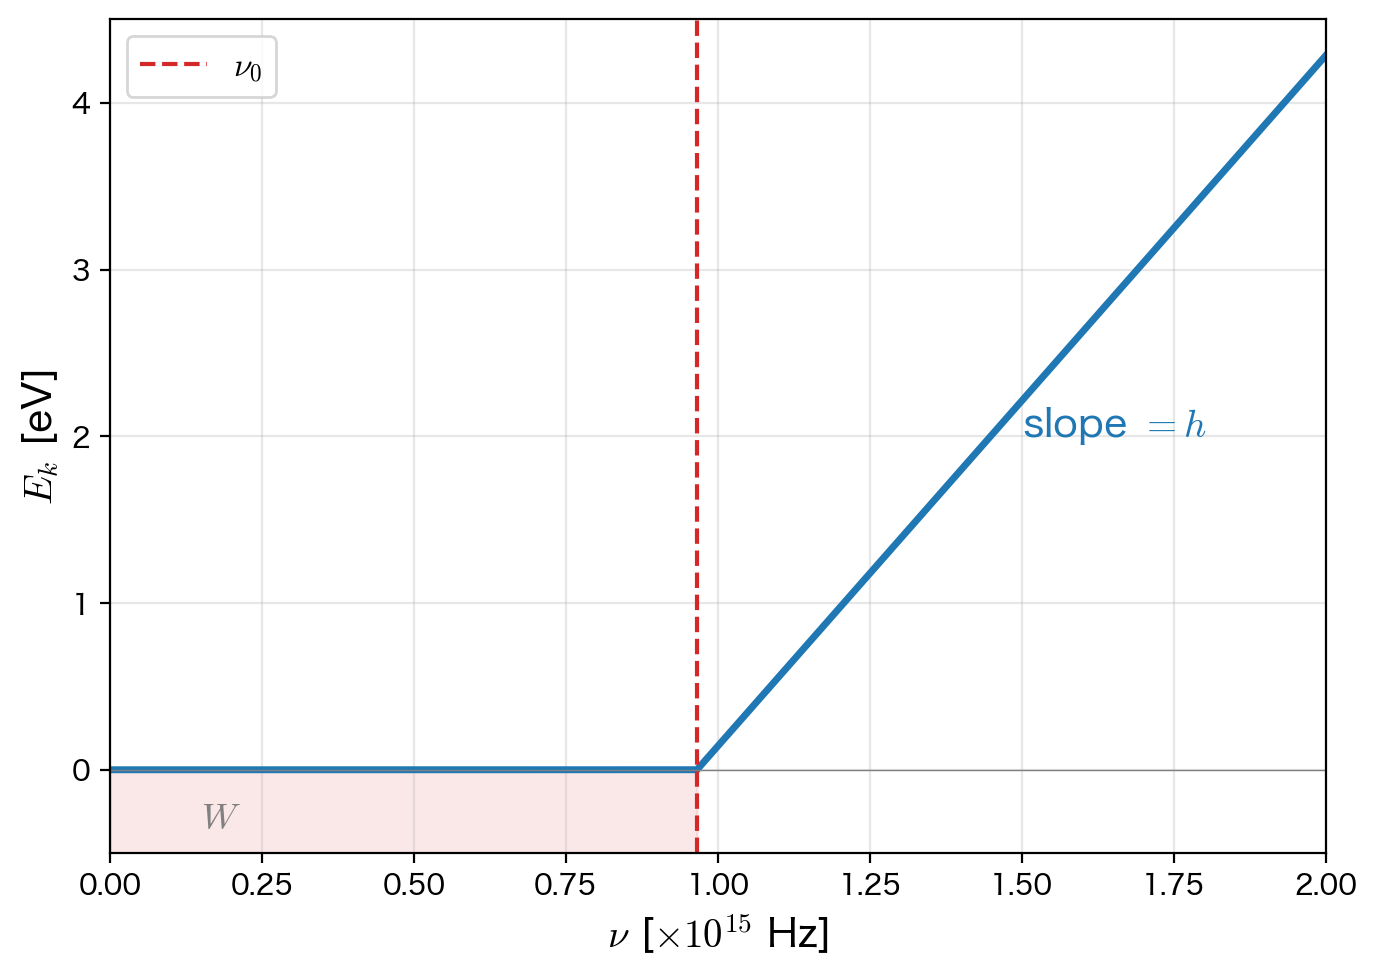
\includegraphics[width=\textwidth]{figures/photoelectric.png}
\end{column}
\end{columns}

\end{frame}

% ============================================================
\begin{frame}{粒子の波動性：ド・ブロイ波}

ここまでで，\textbf{光}は波でもあり粒子でもあることが分かりました。

\vspace{0.3em}
\textbf{de Broglie (1924)} は逆を考えました：

\importantbox{
  光が波と粒子の二重性を持つなら，\\
  \textbf{粒子}（電子など）も波としての性質を持つのではないか？
  \[
    \lambda = \frac{h}{p} = \frac{h}{mv} \qquad \text{（ド・ブロイ波長）}
  \]
}

\vspace{0.3em}
{\small 電子線回折実験 (Davisson--Germer, 1927) で実証。}

\teacher{粒子が波なら，その波を記述する方程式が必要 → Schrödinger方程式へ。}
\end{frame}

% %%%%%%%%%%%%%%%%%%%%%%%%%%%%%%%%%%%%%%%%%%%%%%%%%%%%%%%%%%%%
\section{Schrödinger方程式はどこから来るのか}
% %%%%%%%%%%%%%%%%%%%%%%%%%%%%%%%%%%%%%%%%%%%%%%%%%%%%%%%%%%%%

% ============================================================
\begin{frame}{出発点：粒子を波として書く}

粒子が波なら，波の式（\textbf{波動関数}）で書けるはずです。

\vspace{0.3em}
一般的な平面波：
\[
  \Psi(x,t) = A \exp\!\left[2\pi i\!\left(\frac{x}{\lambda} - \nu t\right)\right]
\]

ここに de Broglie の関係（$\lambda = h/p$，$E = h\nu$）を代入すると：

\[
  \lambda = \frac{h}{p} = \frac{2\pi\hbar}{p}, \qquad
  \nu = \frac{E}{h}
\]

\importantbox{
  $\displaystyle \Psi(x,t) = A \exp\!\left[\frac{i}{\hbar}(px - Et)\right]$
}

{\small $\hbar \equiv h/(2\pi)$：ディラック定数（換算Planck定数）}

\vspace{0.3em}
\teacher{この式が全ての出発点です。ここから微分で演算子を導きます。}
\end{frame}

% ============================================================
\begin{frame}{なぜ微分すると運動量が出るのか}

$\Psi = A\exp\!\bigl[\tfrac{i}{\hbar}(px - Et)\bigr]$ を$x$で偏微分してみましょう：

\[
  \frac{\partial \Psi}{\partial x}
  = A \cdot \frac{ip}{\hbar} \cdot \exp\!\left[\frac{i}{\hbar}(px - Et)\right]
  = \frac{ip}{\hbar}\,\Psi
\]

両辺に$\dfrac{\hbar}{i}$をかけると：

\[
  \frac{\hbar}{i}\frac{\partial \Psi}{\partial x} = p\,\Psi
\]

\teacher{$x$で微分するという「操作」が，$p$という「値」を取り出した！\\
このような操作を\textbf{演算子}，取り出された値を\textbf{固有値}と呼びます。}

\importantbox{
  \textbf{運動量演算子：}\quad $\hat{p} = \dfrac{\hbar}{i}\dfrac{\partial}{\partial x} = -i\hbar\dfrac{\partial}{\partial x}$
}
\end{frame}

% ============================================================
\begin{frame}{同様に，エネルギー演算子}

今度は$t$で偏微分してみます：

\[
  \frac{\partial \Psi}{\partial t}
  = A \cdot \frac{(-iE)}{\hbar} \cdot \exp\!\left[\frac{i}{\hbar}(px - Et)\right]
  = \frac{-iE}{\hbar}\,\Psi
\]

整理すると：

\[
  i\hbar\frac{\partial \Psi}{\partial t} = E\,\Psi
\]

\importantbox{
  \textbf{エネルギー演算子：}\quad $\hat{E} = i\hbar\dfrac{\partial}{\partial t}$
}

\vspace{0.3em}
\teacher{まとめると：\\
$x$で微分 → 運動量$p$が出る　／　$t$で微分 → エネルギー$E$が出る\\
これが量子力学の\textbf{演算子と固有値}の考え方です。}
\end{frame}

% ============================================================
\begin{frame}{Schrödinger方程式の完成}

古典力学：$E = p^2/(2m) + V(x)$ に演算子を代入：

$p \to \hat{p} = -i\hbar\partial_x$，\;$E \to \hat{E} = i\hbar\partial_t$

\[
  \hat{H} = -\frac{\hbar^2}{2m}\frac{\partial^2}{\partial x^2} + V(x)
  \quad \text{（\textbf{ハミルトニアン}：全エネルギーの演算子）}
\]

\importantbox{
  \textbf{時間依存Schrödinger方程式：}\;
  $\displaystyle \hat{H}\Psi = i\hbar\frac{\partial}{\partial t}\Psi$
}

\teacher{量子力学の全てはこの1本の方程式から出発します。}
\end{frame}

% ============================================================
\begin{frame}{時間に依存しないSchrödinger方程式}

$V(x)$が時間に依存しない場合，変数分離$\Psi = \psi(x)\cdot T(t)$で：
\[
  \underbrace{\frac{1}{\psi}\hat{H}\psi}_{x\text{のみ}}
  = \underbrace{\frac{i\hbar}{T}\frac{dT}{dt}}_{t\text{のみ}}
  = E \quad (\text{定数})
\]

\importantbox{
  \textbf{時間非依存Schrödinger方程式：}\;
  $\displaystyle -\frac{\hbar^2}{2m}\frac{d^2\psi}{dx^2} + V(x)\psi = E\psi$
}

時間部分：$T(t) = e^{-iEt/\hbar}$，全体：$\Psi(x,t) = \psi(x)\,e^{-iEt/\hbar}$

\teacher{入試で「Schrödinger方程式を書け」＝ ほぼこの時間非依存形のこと。}
\end{frame}

% %%%%%%%%%%%%%%%%%%%%%%%%%%%%%%%%%%%%%%%%%%%%%%%%%%%%%%%%%%%%
\section{どうやって解くのか（変数分離法）}
% %%%%%%%%%%%%%%%%%%%%%%%%%%%%%%%%%%%%%%%%%%%%%%%%%%%%%%%%%%%%

% ============================================================
\begin{frame}{数学の準備：なぜ波動方程式を先に学ぶのか}

Schrödinger方程式は\textbf{二階偏微分方程式}の一種です。

\vspace{0.3em}
\teacher{解き方のパターンを掴むために，\\
もっと馴染みのある\textbf{弦の振動}（波動方程式）で練習しましょう。\\
解法の手順はSchrödinger方程式と\alert{全く同じ}です。}

\vspace{0.3em}
\textbf{波動方程式：}
\[
  \frac{\partial^2 u}{\partial t^2} = c^2 \frac{\partial^2 u}{\partial x^2}
  \qquad (0 < x < L)
\]

\textbf{解法の手順：}
\begin{enumerate}
  \item $u(x,t) = f(x)\cdot g(t)$ と置く（\textbf{変数分離}）
  \item $x$だけの式と$t$だけの式に分離 → 各々を常微分方程式として解く
  \item \textbf{境界条件}を適用 → 解の形が確定
  \item 許されるエネルギー（固有値）が\alert{離散的}に決まる
\end{enumerate}
\end{frame}

% ============================================================
\begin{frame}{変数分離の実行}

$u = f(x)g(t)$ を波動方程式に代入して，両辺を$f\cdot g$で割ると：

\[
  \frac{1}{c^2 g}\frac{d^2 g}{dt^2}
  = \frac{1}{f}\frac{d^2 f}{dx^2}
\]

\teacher{左辺は$t$だけ，右辺は$x$だけの関数です。\\
$x$と$t$は独立に動くのに等式が成り立つ → \alert{両辺は定数}でなければならない。}

\vspace{0.3em}
この定数を$\lambda$と置くと，$x$部分だけ取り出せます：

\importantbox{
  $\dfrac{d^2 f}{dx^2} = \lambda f(x)$
  \quad ← 二階の常微分方程式（\textbf{固有値問題}）
}

\teacher{$\lambda$の値によって解の形が全く変わります。\\
次のスライドで場合分けを見ましょう。}
\end{frame}

% ============================================================
\begin{frame}{$\lambda$の符号で解が決まる}

\begin{columns}[T]
\begin{column}{0.5\textwidth}
  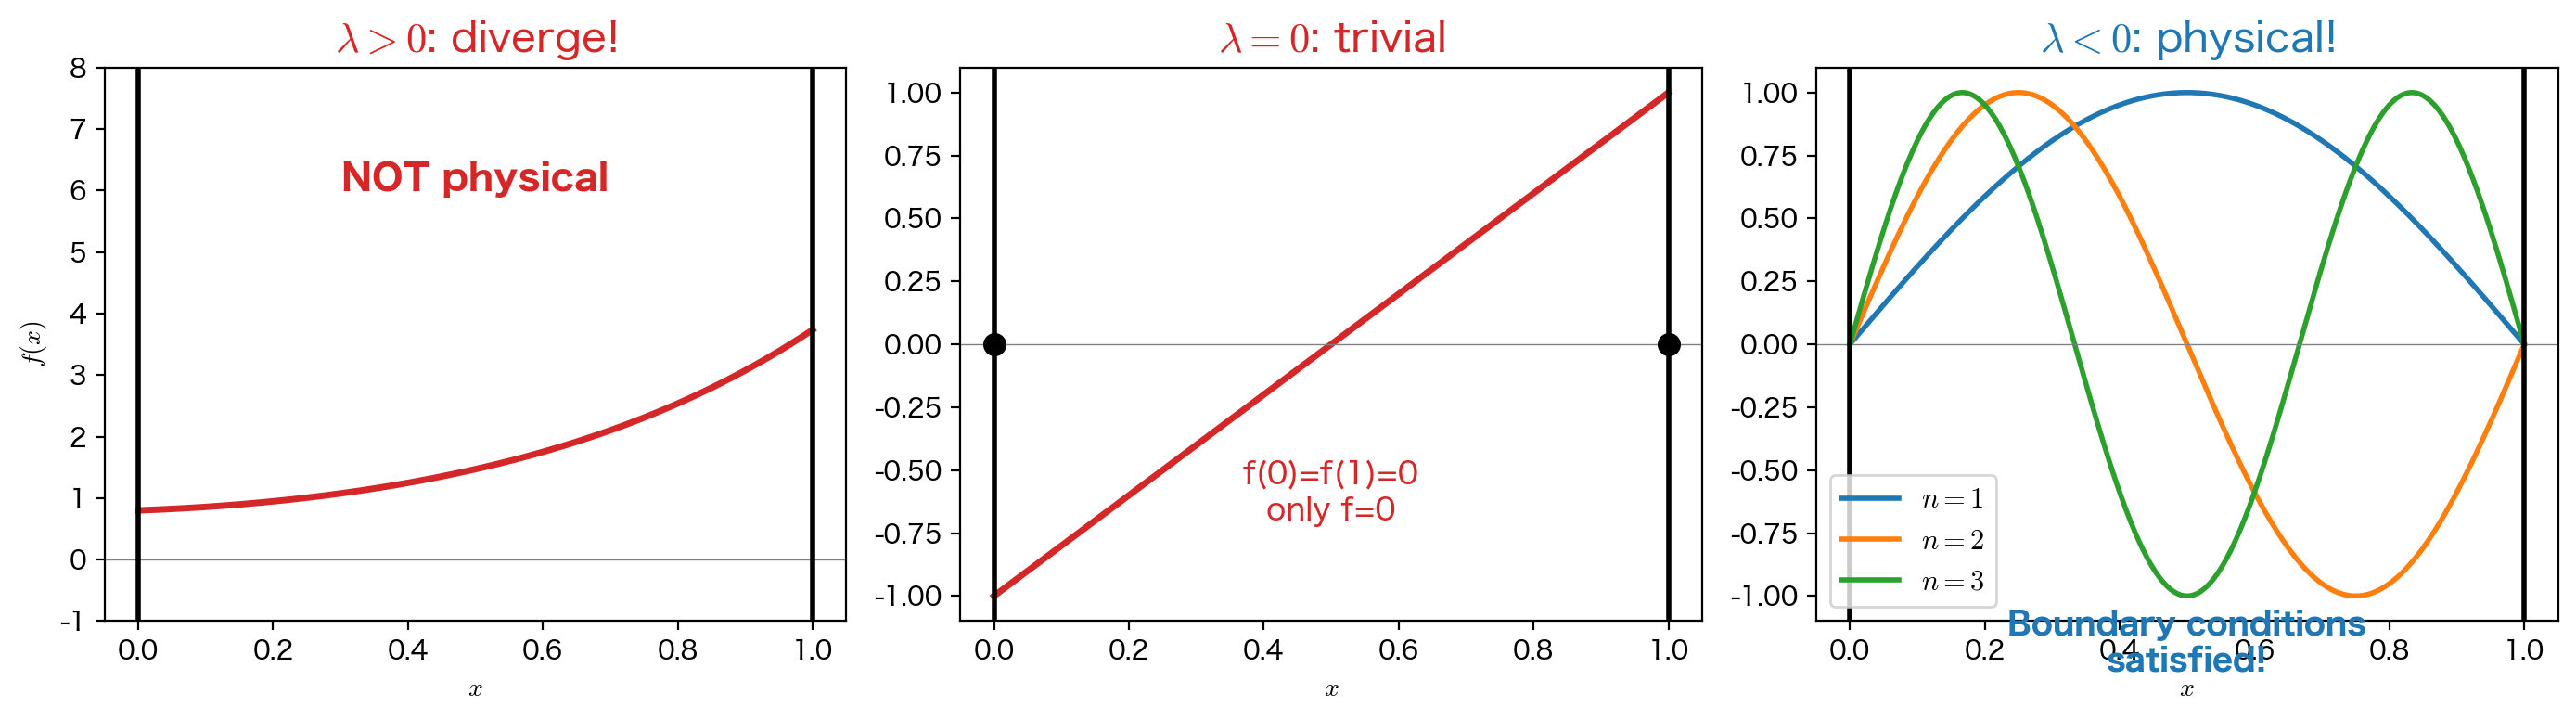
\includegraphics[width=0.95\textwidth]{figures/lambda_cases.png}
\end{column}
\begin{column}{0.5\textwidth}
\textbf{\color{alertred}$\lambda > 0$：}
指数関数 → 発散 → \textbf{不適}

\vspace{0.3em}
\textbf{\color{alertred}$\lambda = 0$：}
直線 → 自明解のみ → \textbf{不適}

\vspace{0.3em}
\textbf{\color{darkblue}$\lambda < 0$：}
三角関数（$\sin$, $\cos$）→ 境界条件を満たせる！
\end{column}
\end{columns}

\vspace{0.3em}
\teacher{$\lambda < 0$のみ物理的に正しい。}
境界条件$f(0) = 0$, $f(L) = 0$を適用：
\[
  \boxed{f_n(x) = D\sin\!\left(\frac{n\pi x}{L}\right), \quad n = 1,2,3,\ldots}
\]
\end{frame}

% %%%%%%%%%%%%%%%%%%%%%%%%%%%%%%%%%%%%%%%%%%%%%%%%%%%%%%%%%%%%
\section{井戸型ポテンシャル}
% %%%%%%%%%%%%%%%%%%%%%%%%%%%%%%%%%%%%%%%%%%%%%%%%%%%%%%%%%%%%

% ============================================================
\begin{frame}{箱の中の粒子（Particle in a Box）}

\begin{columns}[c]
\begin{column}{0.4\textwidth}
  \begin{tikzpicture}[scale=0.75]
    \fill[pattern=north east lines, pattern color=gray] (-0.5,0) rectangle (0,2.5);
    \fill[pattern=north east lines, pattern color=gray] (3.5,0) rectangle (4,2.5);
    \draw[very thick] (0,2.5) -- (0,0) -- (3.5,0) -- (3.5,2.5);
    \fill[yellow!30, opacity=0.5] (0,0) rectangle (3.5,2.5);
    \node[below] at (0,-0.1) {\small$0$};
    \node[below] at (3.5,-0.1) {\small$a$};
    \node at (1.75,1.2) {$V=0$};
    \node at (-0.8,1.2) {\small$\infty$};
    \node at (4.3,1.2) {\small$\infty$};
  \end{tikzpicture}
\end{column}
\begin{column}{0.6\textwidth}
  $V(x) = 0\;(0 \leq x \leq a)$，それ以外$V = \infty$

  壁の外：$\psi = 0$（存在確率ゼロ）

  \vspace{0.3em}
  箱の中（$V = 0$）のSchrödinger方程式：
  \[
    -\frac{\hbar^2}{2m}\frac{d^2\psi}{dx^2} = E\psi
  \]
\end{column}
\end{columns}

$k \equiv \sqrt{2mE/\hbar^2}$ とおくと：
\[
  \frac{d^2\psi}{dx^2} = -k^2\psi
\]

\teacher{波動方程式で練習した$f'' = \lambda f$（$\lambda = -k^2$）と\alert{全く同じ形}！}
\end{frame}

% ============================================================
\begin{frame}{境界条件の適用}

一般解：$\psi(x) = A\cos(kx) + B\sin(kx)$

\vspace{0.3em}
\textbf{境界条件①：} $\psi(0) = 0$
\[
  \psi(0) = A\cos(0) + B\sin(0) = A = 0
\]

\teacher{$A = 0$なので，$\psi(x) = B\sin(kx)$だけが残ります。}

\vspace{0.3em}
\textbf{境界条件②：} $\psi(a) = 0$
\[
  \psi(a) = B\sin(ka) = 0
\]

$B = 0$だと$\psi = 0$（粒子が存在しない）→ 意味がないので$B \neq 0$。\\
したがって：
\[
  \sin(ka) = 0 \quad \Longrightarrow \quad ka = n\pi \quad (n = 1, 2, 3, \ldots)
\]

\importantbox{
  $k = \dfrac{n\pi}{a}$，\qquad $\psi_n(x) = B\sin\!\left(\dfrac{n\pi x}{a}\right)$
}

{\small ※ $n = 0$は$\psi = 0$（粒子不存在）なので除外。}
\end{frame}

% ============================================================
\begin{frame}{規格化：係数$B$を決める}

\teacher{「粒子がどこかに必ず存在する」→ 確率の総和$= 1$で$B$が決まる。}

\[
  \int_0^a |\psi_n|^2\,dx = B^2 \int_0^a \sin^2\!\left(\frac{n\pi x}{a}\right)dx = 1
\]

半角公式 $\sin^2\theta = (1 - \cos 2\theta)/2$ で積分：
\[
  B^2 \int_0^a \frac{1 - \cos(2n\pi x/a)}{2}\,dx
  = B^2 \left[\frac{x}{2} - \frac{a}{4n\pi}\sin\!\left(\frac{2n\pi x}{a}\right)\right]_0^a
  = B^2 \cdot \frac{a}{2}
\]

$\therefore\; B = \sqrt{2/a}$

\importantbox{
  $\boxed{\psi_n(x) = \sqrt{\dfrac{2}{a}}\sin\!\left(\dfrac{n\pi x}{a}\right), \quad n = 1, 2, 3, \ldots}$
}
\end{frame}

% ============================================================
\begin{frame}{エネルギー固有値}

$k = \sqrt{2mE/\hbar^2} = n\pi/a$ から$E$について解くと：

\importantbox{
  \[
    \boxed{E_n = \frac{n^2\pi^2\hbar^2}{2ma^2} = \frac{n^2 h^2}{8ma^2}, \qquad n = 1, 2, 3, \ldots}
  \]
}

\teacher{エネルギーは連続ではなく，$n = 1, 2, 3, \ldots$の\alert{飛び飛びの値}しか取れません。}

\vspace{0.3em}
\begin{center}
\begin{tabular}{lcc}
  \toprule
  & \textbf{古典力学} & \textbf{量子力学} \\
  \midrule
  エネルギー & 連続（任意の値） & \alert{離散的}（$n^2$に比例） \\
  最低エネルギー & $E = 0$（静止可能） & $E_1 > 0$（\alert{零点エネルギー}） \\
  \bottomrule
\end{tabular}
\end{center}
\end{frame}

% ============================================================
\begin{frame}{量子効果はどのくらい大きいか}

\textbf{数値例：}電子（$m = \SI{9.11e-31}{kg}$）を$a = \SI{1}{nm}$の箱に入れると
\[
  E_1 = \frac{(\SI{6.626e-34}{})^2}{8 \times \SI{9.11e-31}{} \times (\SI{1e-9}{})^2}
  \approx \SI{0.376}{eV}
\]

室温の熱エネルギー：$k_\mathrm{B}T \approx \SI{0.025}{eV}$

\vspace{0.3em}
\importantbox{
  $E_1 \approx \SI{0.376}{eV} \gg k_\mathrm{B}T \approx \SI{0.025}{eV}$\\[4pt]
  → 原子・分子スケールでは量子効果は\alert{無視できない}！
}

\teacher{逆にマクロな物体（$m$が大きい，$a$が大きい）では$E_1 \approx 0$\\
→ エネルギーが事実上連続 → 古典力学で十分。}
\end{frame}

% %%%%%%%%%%%%%%%%%%%%%%%%%%%%%%%%%%%%%%%%%%%%%%%%%%%%%%%%%%%%
\section{解から何が分かるのか}
% %%%%%%%%%%%%%%%%%%%%%%%%%%%%%%%%%%%%%%%%%%%%%%%%%%%%%%%%%%%%

% ============================================================
\begin{frame}{波動関数の物理的意味（Bornの確率解釈）}

\teacher{$\psi_n(x)$が求まりましたが，これは何を意味するのでしょうか？}

\vspace{0.3em}
\textbf{Born (1926)} の解釈：

\importantbox{
  $|\psi(x)|^2\,dx$ = 位置$x$〜$x + dx$に粒子を見出す\textbf{確率}
}

波動関数が満たすべき条件：
\begin{enumerate}
  \item \textbf{規格化：}$\int|\psi|^2 dx = 1$（どこかに必ずいる）
  \item \textbf{連続：}$\psi(x)$はなめらか
  \item \textbf{一価：}各点で値が一つ
  \item \textbf{有界：}$\psi(x)$は有限
\end{enumerate}

\vspace{0.3em}
\teacher{$\psi$自体は複素数で直接の意味はありませんが，\\
$|\psi|^2$は「粒子をそこで見つける確率」という明確な物理量です。}
\end{frame}

% ============================================================
\begin{frame}{波動関数と存在確率を見てみよう}

\begin{columns}[T]
\begin{column}{0.5\textwidth}
  \centering
  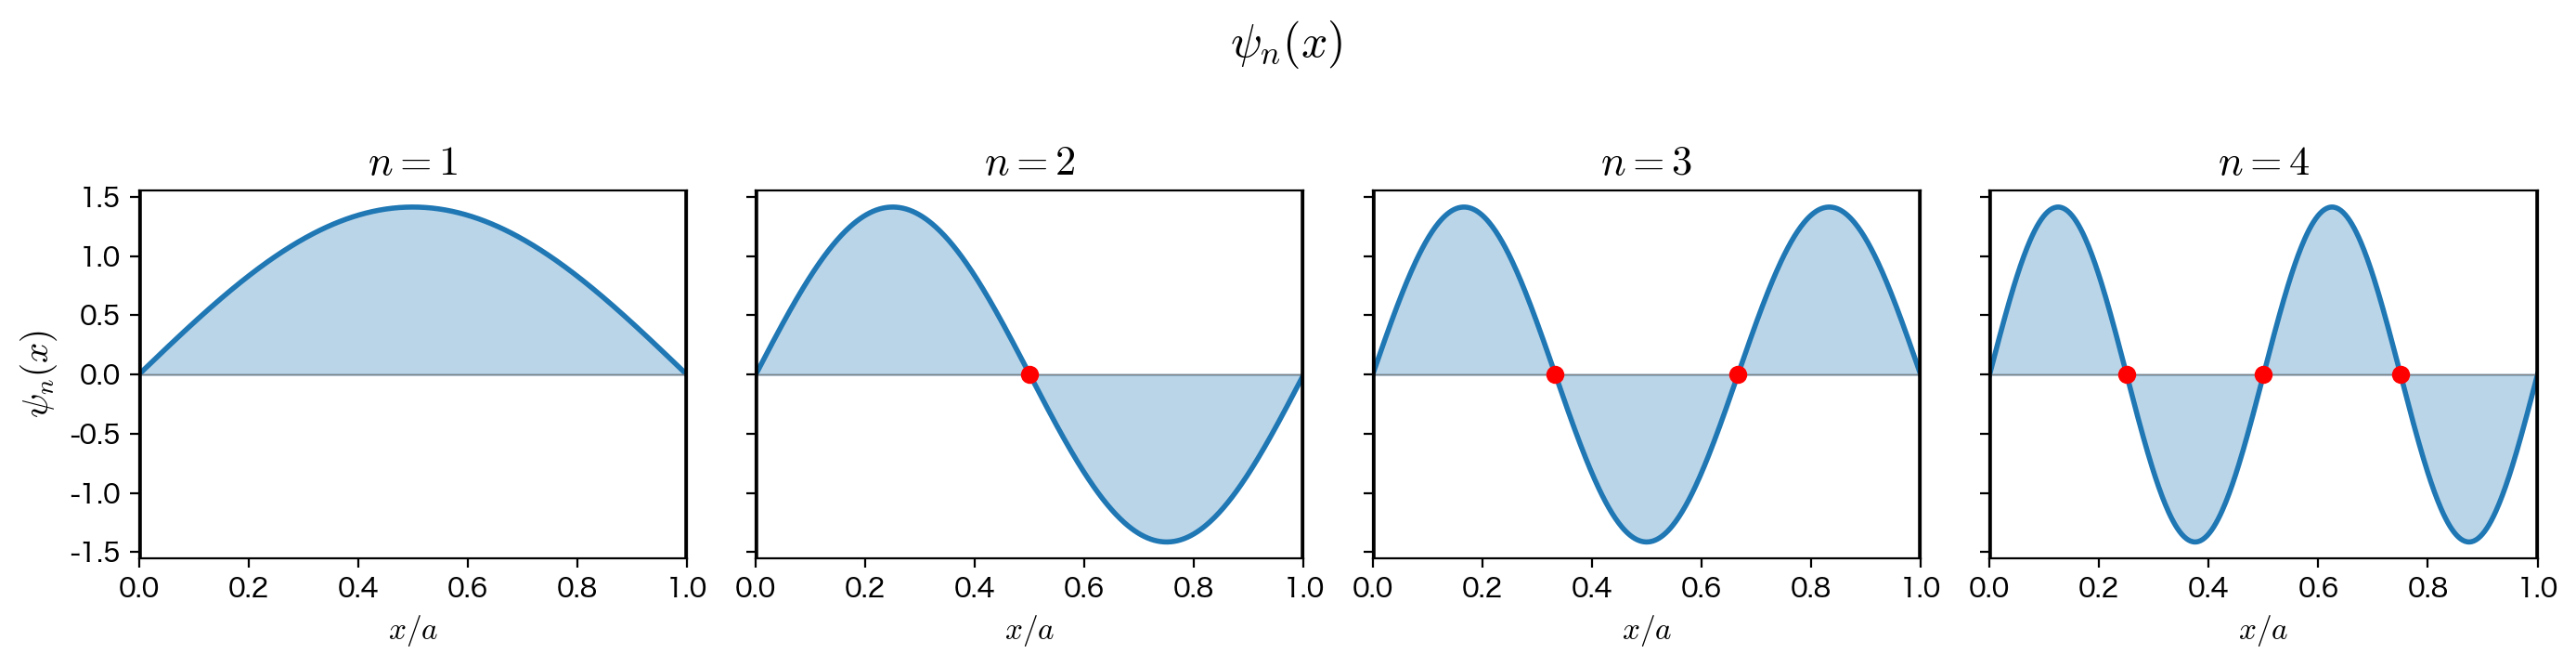
\includegraphics[width=\textwidth]{figures/wavefunctions.png}\\
  {\small $\psi_n(x)$：赤丸＝\textbf{節}（$\psi = 0$の点）}
\end{column}
\begin{column}{0.5\textwidth}
  \centering
  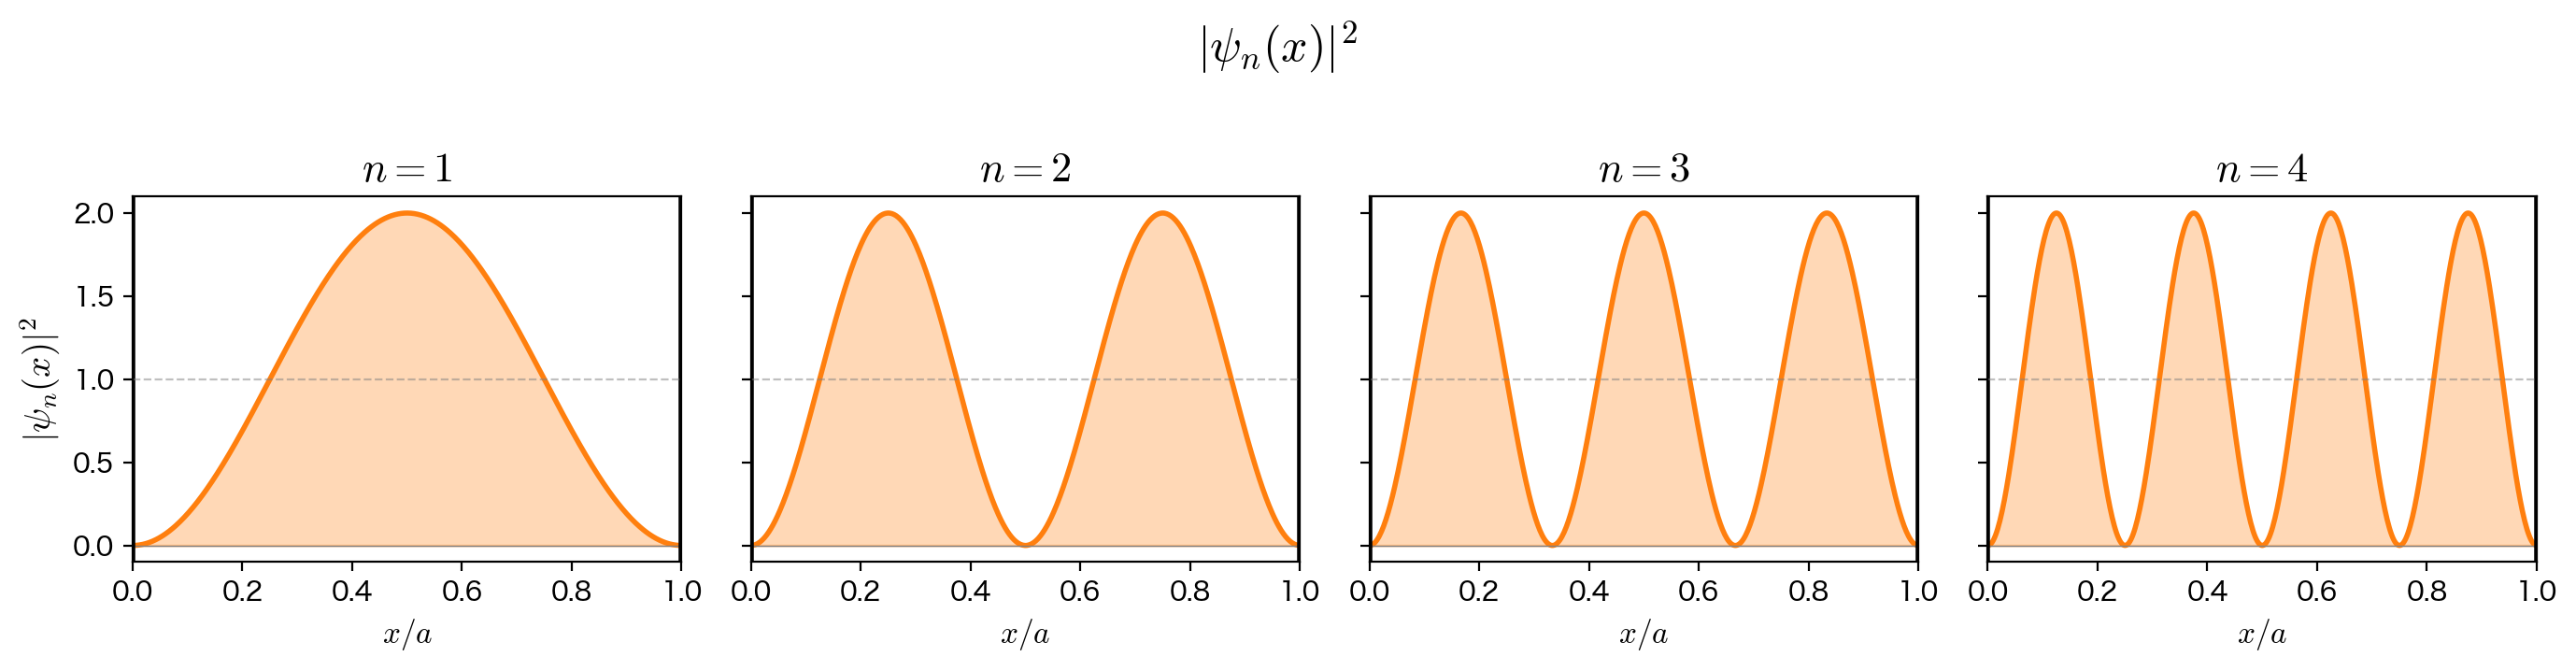
\includegraphics[width=\textwidth]{figures/probability_density.png}\\
  {\small $|\psi_n|^2$：灰破線＝古典極限（一様分布$1/a$）}
\end{column}
\end{columns}

\vspace{0.3em}
\teacher{図から読み取れること：}
\begin{itemize}
  \item $n = 1$：箱の中央に最も存在しやすい
  \item $n = 2$：中央で$|\psi|^2 = 0$（\alert{そこには絶対にいない}！）
  \item 節の数 $= n - 1$ 個
  \item $n$が大きくなると振動が激しくなる
\end{itemize}
\end{frame}

% ============================================================
\begin{frame}{エネルギー準位図}

\begin{columns}[c]
\begin{column}{0.4\textwidth}
  \centering
  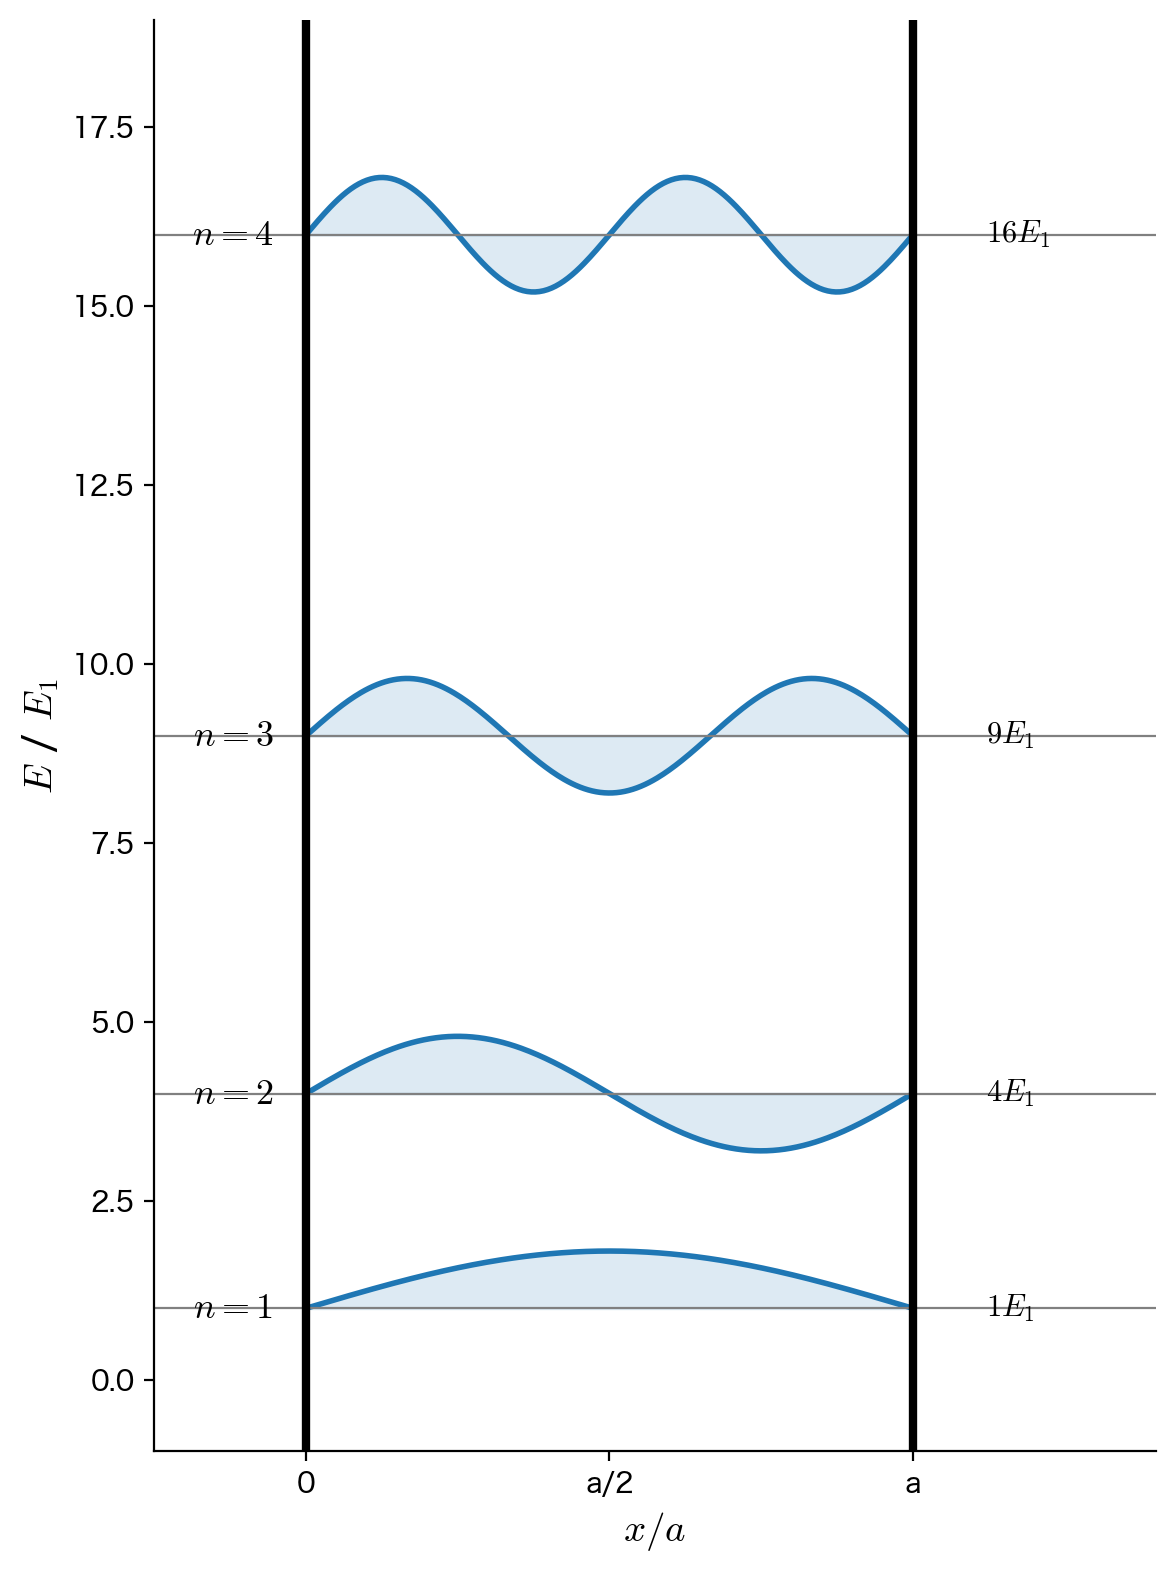
\includegraphics[width=0.95\textwidth]{figures/energy_levels_with_psi.png}
\end{column}
\begin{column}{0.6\textwidth}
  $E_n = n^2 E_1$，\quad $E_1 = h^2/(8ma^2)$

  \vspace{0.3em}
  \begin{tabular}{cccc}
    \toprule
    $n$ & $E_n/E_1$ & 節の数 & 備考 \\
    \midrule
    1 & 1 & 0 & ← \textbf{基底状態} \\
    2 & 4 & 1 & \\
    3 & 9 & 2 & \\
    4 & 16 & 3 & \\
    \bottomrule
  \end{tabular}

  \vspace{0.3em}
  \textbf{規則：}
  \begin{itemize}
    \item 節の数 $= n - 1$
    \item $\Delta E = E_{n+1} - E_n = (2n+1)E_1$\\
      → $n$が大きいほど間隔が\textbf{広がる}
  \end{itemize}
\end{column}
\end{columns}
\end{frame}

% ============================================================
\begin{frame}{零点エネルギー}

\teacher{$n = 0$が許されないということは，\\
粒子は完全に静止できない＝エネルギーがゼロにならないということです。}

\[
  E_1 = \frac{h^2}{8ma^2} \neq 0 \qquad \text{（\textbf{零点エネルギー}）}
\]

\vspace{0.3em}
\textbf{\color{accent}なぜか？ → Heisenbergの不確定性原理で説明できます：}
\[
  \Delta x \cdot \Delta p \geq \frac{\hbar}{2}
\]

\begin{itemize}
  \item 箱に閉じ込める → 位置の不確定さ$\Delta x \leq a$
  \item すると運動量の不確定さ$\Delta p \geq \hbar/(2a)$
  \item 運動量がゼロにならない → エネルギーもゼロにならない
\end{itemize}

\vspace{0.3em}
\teacher{「閉じ込めるほど不確定性原理が効いてエネルギーが上がる」\\
これが量子力学の本質的な結論です。}

\end{frame}

% ============================================================
\begin{frame}{対応原理：古典力学との橋渡し}

\teacher{量子力学と古典力学はどう繋がるのでしょうか？}

\vspace{0.3em}
\textbf{対応原理（Bohr）：}$n \to \infty$で量子力学は古典力学に一致する。

\begin{center}
  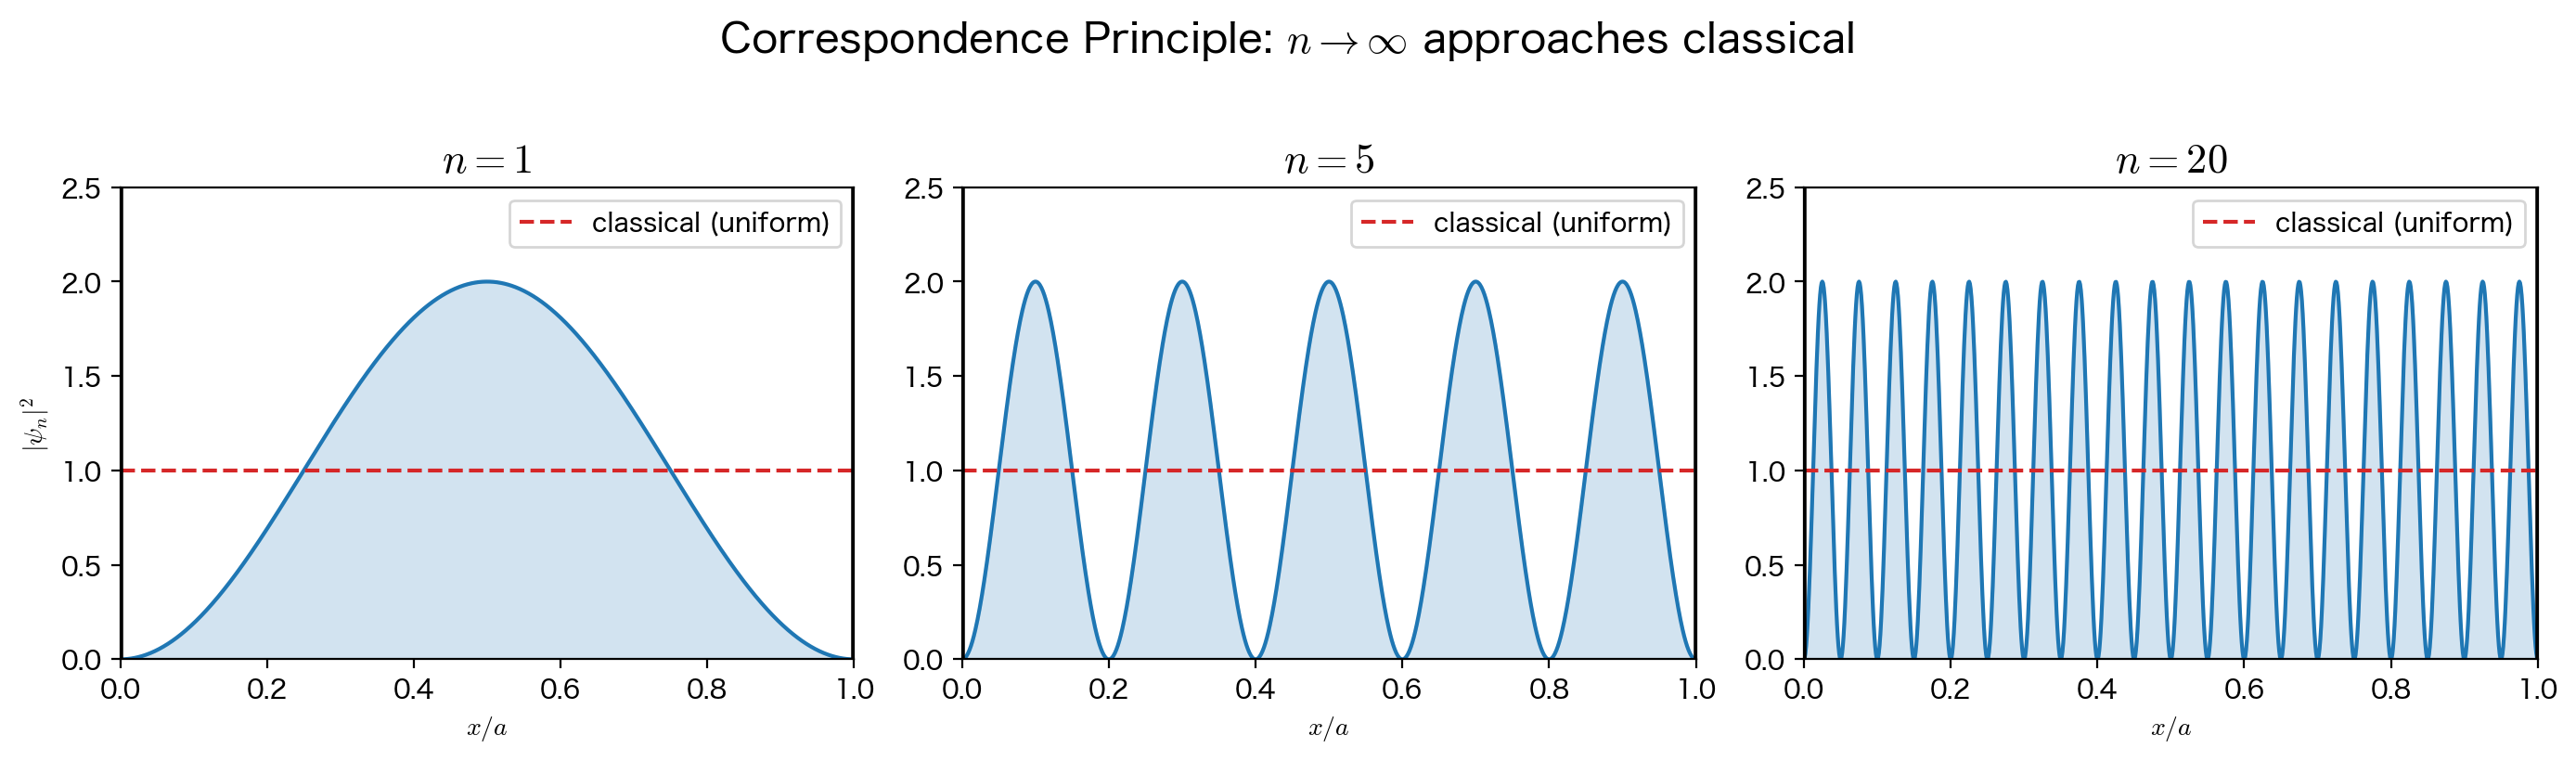
\includegraphics[width=0.65\textwidth]{figures/correspondence.png}
\end{center}

\vspace{-0.5em}
\begin{itemize}
  \item $n = 1$：中央に偏る → 古典力学と異なる
  \item $n = 20$：平均するとほぼ一様 → \textbf{古典的！}
  \item $\Delta E / E_n = (2n+1)/n^2 \to 0$（$n \to \infty$）→ 事実上連続
\end{itemize}
\end{frame}

% %%%%%%%%%%%%%%%%%%%%%%%%%%%%%%%%%%%%%%%%%%%%%%%%%%%%%%%%%%%%
\section{応用：共役ポリエン}
% %%%%%%%%%%%%%%%%%%%%%%%%%%%%%%%%%%%%%%%%%%%%%%%%%%%%%%%%%%%%

% ============================================================
\begin{frame}{共役ポリエンの$\pi$電子モデル}

\teacher{最後に，化学への応用を見ましょう。\\
共役ポリエンの$\pi$電子は「箱の中の粒子」で近似できます。}

\vspace{0.3em}
\textbf{モデル：}
\begin{itemize}
  \item $\pi$電子は分子骨格に沿って自由に動ける → 「箱」
  \item 箱の長さ$a \approx$（結合の数）$\times$（C--C結合長 $\approx \SI{0.14}{nm}$）
  \item Pauliの排他原理：各準位に電子は最大2個（$\uparrow\downarrow$）
\end{itemize}

\vspace{0.3em}
\textbf{用語：}
\begin{itemize}
  \item \textbf{HOMO}：電子が入っている最も高い準位
  \item \textbf{LUMO}：電子が入っていない最も低い準位
  \item 光吸収 ＝ 電子がHOMO → LUMOに遷移
\end{itemize}
\end{frame}

% ============================================================
\begin{frame}{ブタジエンの吸収波長を計算する}

\begin{columns}[c]
\begin{column}{0.6\textwidth}
\textbf{ブタジエン}（4個の$\pi$電子，$a \approx \SI{0.42}{nm}$）

$n=1$に2個，$n=2$に2個 → HOMO: $n=2$，LUMO: $n=3$

\vspace{0.3em}
HOMO→LUMO遷移（$n = 2 \to 3$）：
\[
  \Delta E = 5 \cdot \frac{h^2}{8ma^2} \approx \SI{1.7e-18}{J}
\]
\[
  \lambda = hc/\Delta E \approx \SI{117}{nm}
\]
{\small （実測$\approx \SI{217}{nm}$：モデルの限界）}
\end{column}
\begin{column}{0.4\textwidth}
  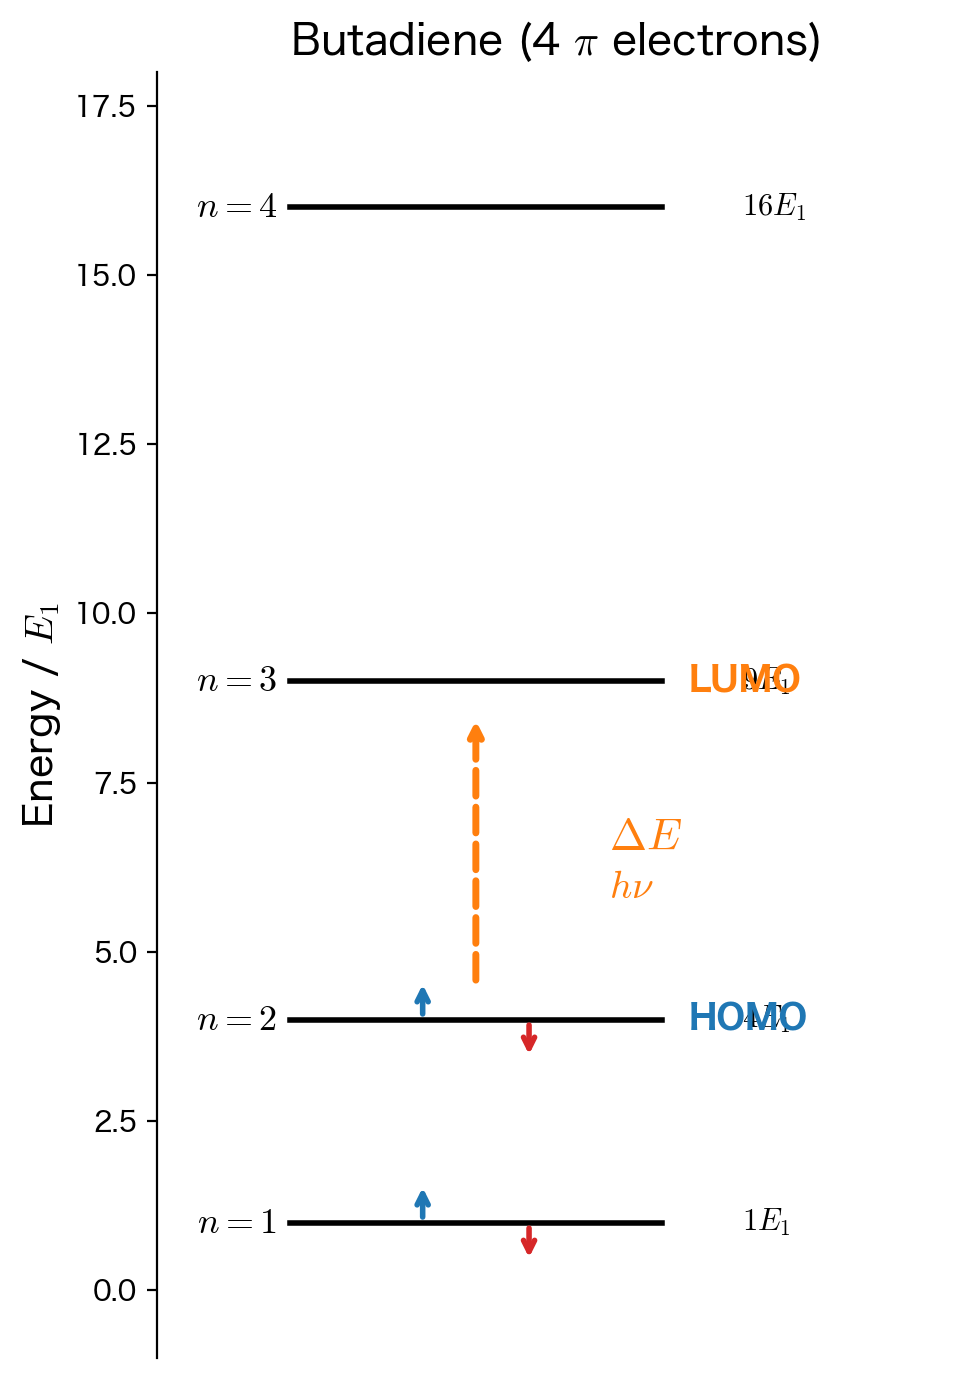
\includegraphics[width=0.85\textwidth]{figures/butadiene_levels.png}
\end{column}
\end{columns}
\end{frame}

% ============================================================
\begin{frame}{共役の長さと色の関係}

\importantbox{
  共役系が長くなる → $a$が増大 → $\Delta E$が減少 → $\lambda$が\alert{赤方偏移}
}

\vspace{0.3em}
\begin{center}
\begin{tabular}{lcccc}
  \toprule
  分子 & $\pi$電子数 & HOMO & LUMO & 傾向 \\
  \midrule
  エチレン & 2 & $n=1$ & $n=2$ & 短波長（UV） \\
  ブタジエン & 4 & $n=2$ & $n=3$ & ↓ \\
  ヘキサトリエン & 6 & $n=3$ & $n=4$ & ↓ \\
  $\beta$-カロテン & 22 & $n=11$ & $n=12$ & 可視光（橙色！） \\
  \bottomrule
\end{tabular}
\end{center}

\vspace{0.3em}
\teacher{にんじんが橙色なのは，$\beta$-カロテンの共役系が長くて\\
可視光を吸収するからです。Particle in a Boxで説明できる！}

\vspace{0.3em}
\end{frame}

% %%%%%%%%%%%%%%%%%%%%%%%%%%%%%%%%%%%%%%%%%%%%%%%%%%%%%%%%%%%%
\section{もう一つの重要な例：分子振動}
% %%%%%%%%%%%%%%%%%%%%%%%%%%%%%%%%%%%%%%%%%%%%%%%%%%%%%%%%%%%%

% ============================================================
\begin{frame}{箱の次は「ばね」：調和振動子}

\teacher{井戸型ポテンシャルの次に大事なのが，\textbf{分子の振動}です。\\
二原子分子の結合を「ばね」と見なすと，調和振動子になります。}

\vspace{0.3em}
\textbf{ポテンシャル：}
\[
  V^\text{H} = \frac{1}{2}k(R - R_e)^2 = \frac{1}{2}kx^2
\]
{\small $k$：ばね定数，$R_e$：平衡結合距離，$x = R - R_e$：変位}

\vspace{0.3em}
\textbf{時間に依存しないSchrödinger方程式：}
\[
  -\frac{\hbar^2}{2\mu}\frac{d^2\psi}{dx^2} + \frac{1}{2}kx^2\psi = E\psi
\]
{\small $\mu$：\textbf{換算質量}（reduced mass）$= m_1 m_2/(m_1 + m_2)$}

\vspace{0.3em}
\teacher{井戸型と違って$V(x)$が$x^2$に比例するので，解はもっと複雑になります。\\
でも結果はとてもシンプルです。}
\end{frame}

% ============================================================
\begin{frame}{調和振動子のエネルギー準位}

\begin{columns}[c]
\begin{column}{0.45\textwidth}
  \centering
  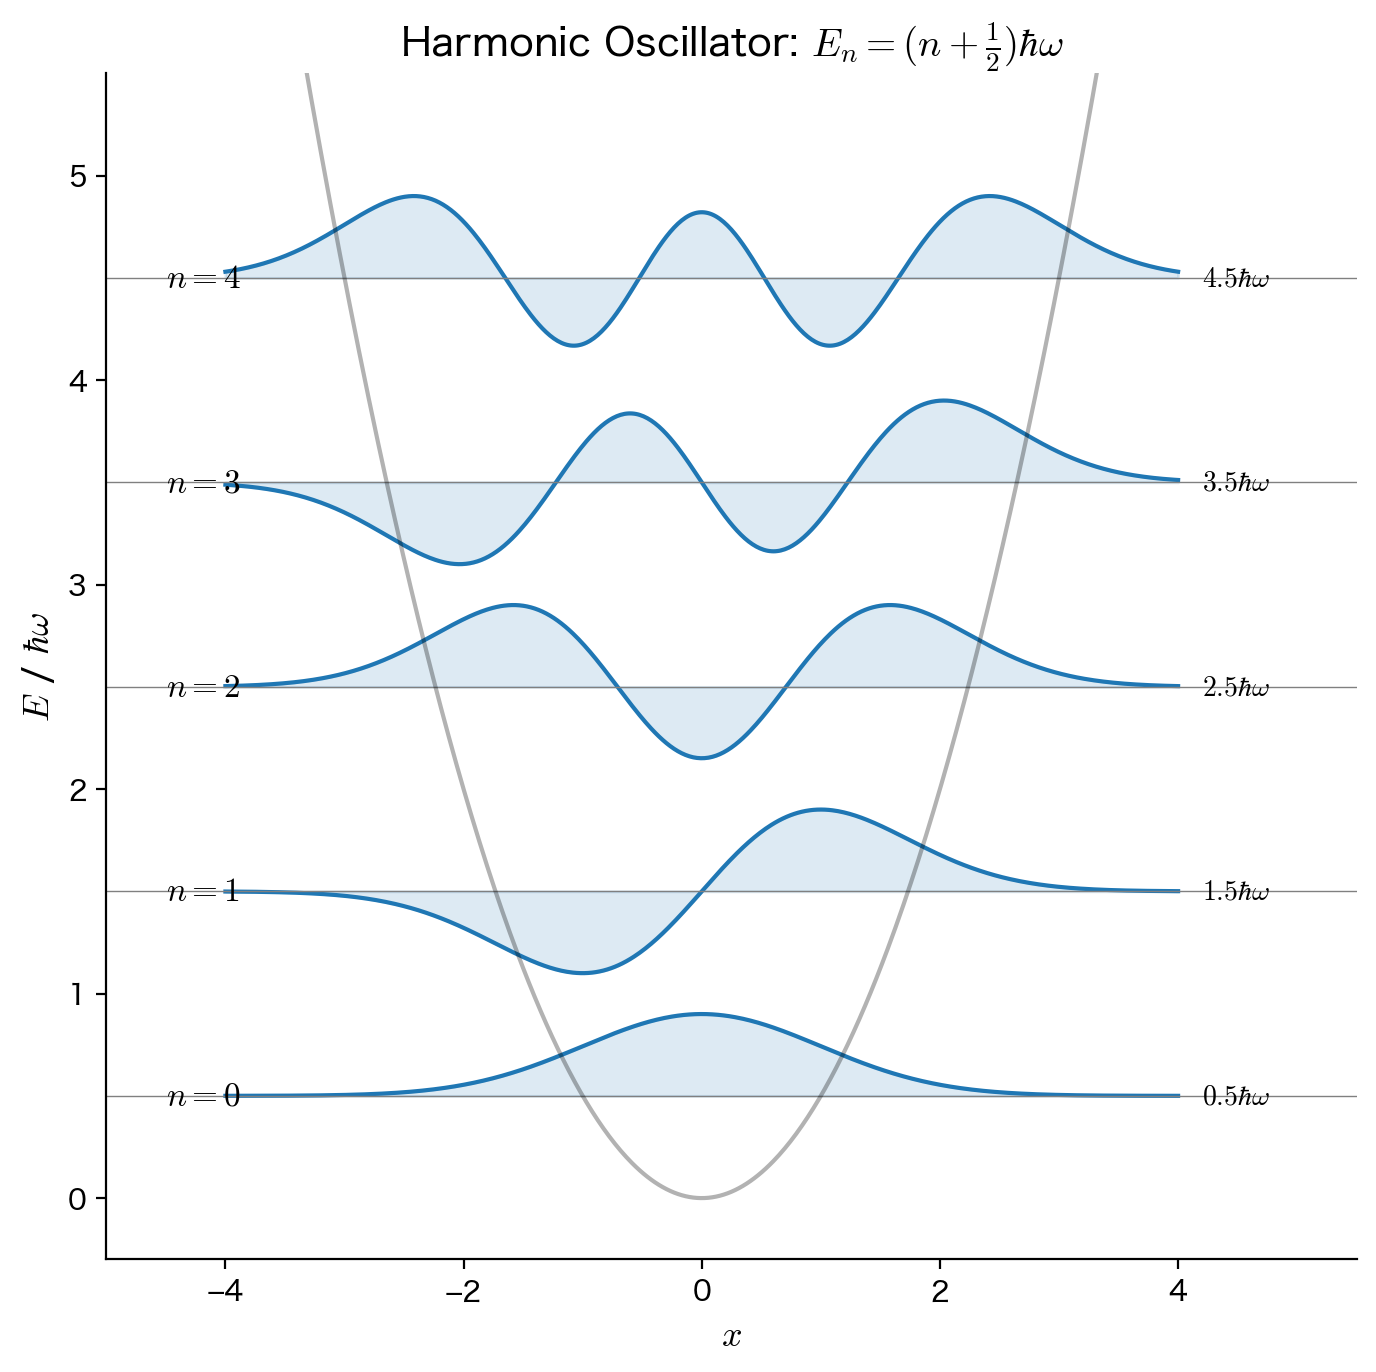
\includegraphics[width=\textwidth]{figures/harmonic_oscillator.png}
\end{column}
\begin{column}{0.55\textwidth}
\importantbox{
  \[
    E_n = \left(n + \frac{1}{2}\right)\hbar\omega, \quad n = 0, 1, 2, \ldots
  \]
  $\omega = \sqrt{k/\mu}$：角振動数
}

\vspace{0.3em}
\textbf{井戸型ポテンシャルとの比較：}

\begin{tabular}{lcc}
  \toprule
  & 井戸型 & 調和振動子 \\
  \midrule
  $E_n$ & $\propto n^2$ & $\propto n$ \\
  間隔 & 不均一 & \alert{等間隔} $\hbar\omega$ \\
  零点E & $E_1 \neq 0$ & $E_0 = \frac{1}{2}\hbar\omega \neq 0$ \\
  量子数 & $n = 1,2,3,\ldots$ & $n = 0,1,2,\ldots$ \\
  \bottomrule
\end{tabular}
\end{column}
\end{columns}

\vspace{0.3em}
\teacher{波数$\tilde{\nu}$で表すと：$E_n = (n+\frac{1}{2})hc\tilde{\nu}$。\\
赤外吸収の波数がそのまま$\tilde{\nu}$に対応します。}
\end{frame}

% ============================================================
\begin{frame}{赤外吸収の選択律}

\teacher{調和振動子のエネルギー間隔は等間隔$\hbar\omega$なので，\\
赤外光を吸収するときの条件はシンプルです。}

\vspace{0.3em}
\textbf{選択律（selection rule）：}
\importantbox{
  $\Delta n = \pm 1$ \quad （基本振動のみ許される）
}

\textbf{赤外吸収のもう一つの条件：}

振動に伴い\textbf{双極子モーメントが変化}すること

\teacher{対称分子（H$_2$, N$_2$）は振動しても双極子が変わらない → 赤外不活性}
\end{frame}

% ============================================================
\begin{frame}{赤外活性と基準振動モード}

\begin{tabular}{lcl}
  \toprule
  分子 & 赤外活性？ & 理由 \\
  \midrule
  HCl, CO, H$_2$O & ○ & 双極子モーメントが変化 \\
  H$_2$, N$_2$, O$_2$ & × & 対称 → 双極子変化なし \\
  CO$_2$（逆対称伸縮） & ○ & 非対称モードで双極子変化 \\
  \bottomrule
\end{tabular}

\vspace{0.6em}
\textbf{基準振動モード数：}
\begin{itemize}
  \item 非直線分子：$3N - 6$
  \item 直線分子：$3N - 5$
\end{itemize}

{\small 例：CO$_2$（直線，$N=3$）→ $3\times3 - 5 = 4$モード}
\end{frame}

% ============================================================
\begin{frame}{換算質量と振動波数の計算}

\teacher{入試では，具体的な分子の赤外吸収波数を計算させる問題がよく出ます。}

\vspace{0.3em}
\textbf{換算質量：}
\[
  \mu = \frac{m_1 m_2}{m_1 + m_2}
\]

\textbf{振動波数：}
\[
  \tilde{\nu} = \frac{1}{2\pi c}\sqrt{\frac{k}{\mu}}
\]

\vspace{0.3em}
\textbf{計算例：}$^{12}$C$^{16}$O（$k = \SI{1855}{N.m^{-1}}$）
\begin{align}
  \mu &= \frac{12 \times 16}{12 + 16} \times \frac{1}{\SI{6.02e23}{}} = \SI{1.14e-26}{kg} \\[4pt]
  \tilde{\nu} &= \frac{1}{2\pi \times \SI{3.00e8}{}}\sqrt{\frac{1855}{\SI{1.14e-26}{}}}
  \approx \SI{2150}{cm^{-1}}
\end{align}
\end{frame}

% ============================================================
\begin{frame}{実在分子：Morseポテンシャル}

\teacher{実際の分子は大きく伸ばすと解離する → 非対称ポテンシャル。}

\begin{columns}[c]
\begin{column}{0.45\textwidth}
  \centering
  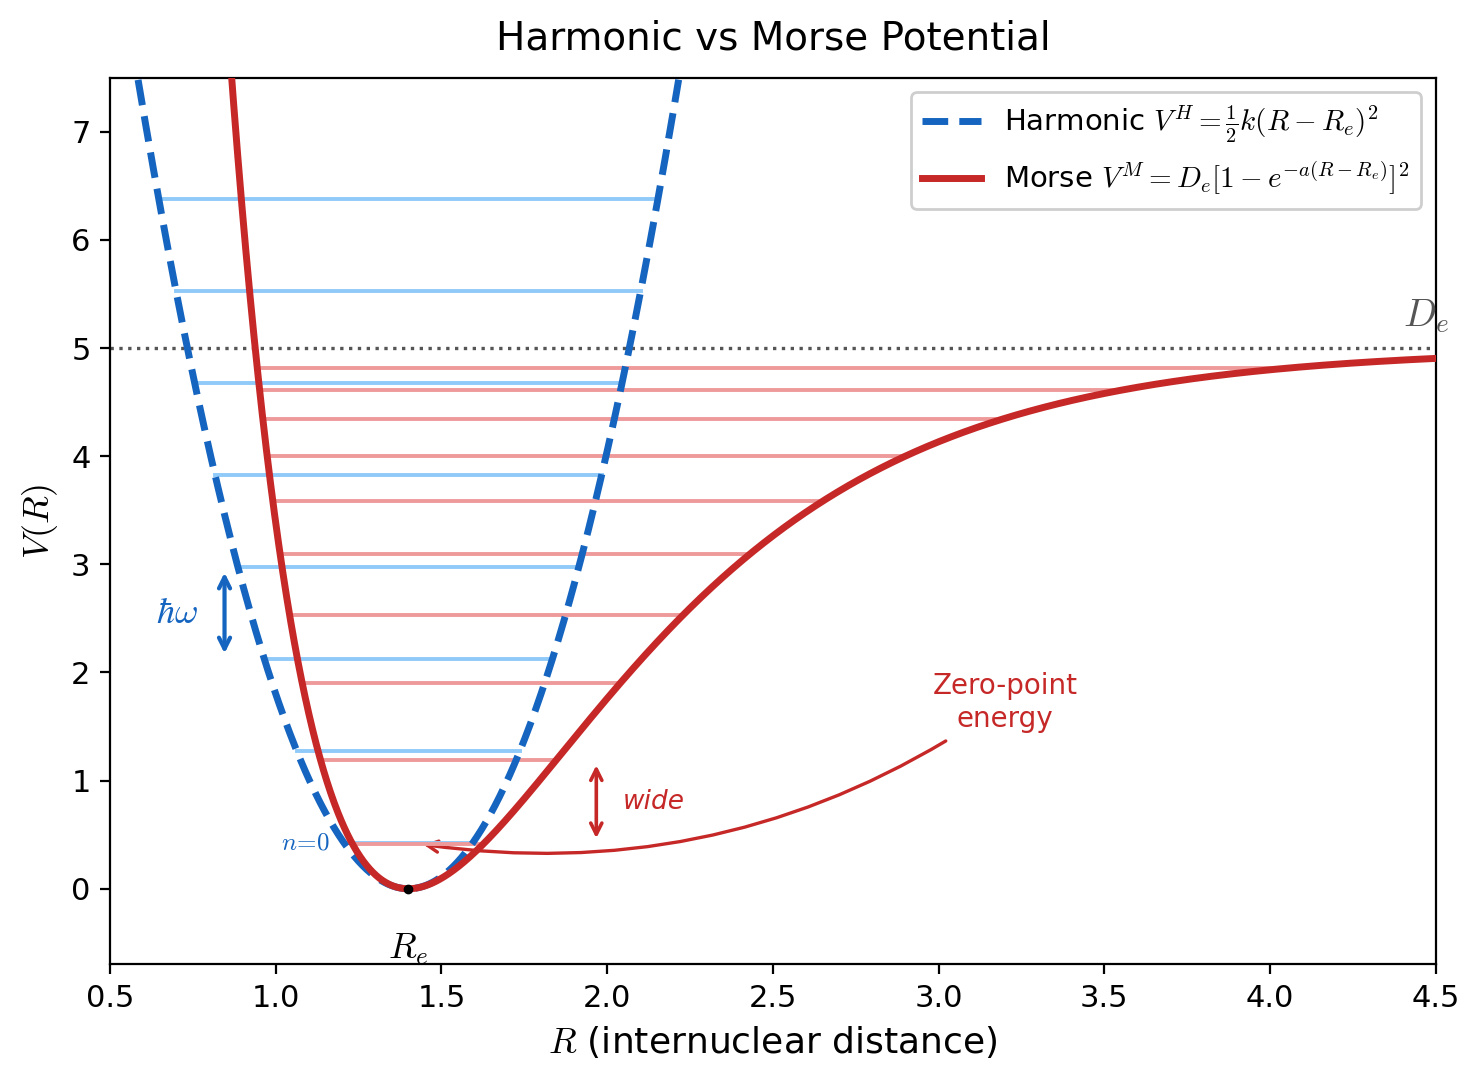
\includegraphics[width=0.95\textwidth]{figures/morse_vs_harmonic.png}
\end{column}
\begin{column}{0.55\textwidth}
$V^\text{M} = D_e[1 - e^{-a(R-R_e)}]^2$\quad{\small ($D_e$：解離エネルギー)}

\vspace{0.2em}
$E_n^\text{M} = E_n^\text{H} - (n+\tfrac{1}{2})^2 \dfrac{hc\tilde{\nu}^2}{4D_e}$

\vspace{0.3em}
\textbf{調和振動子との違い：}
\begin{itemize}
  \item 間隔が$n$とともに\alert{狭くなる}
  \item 有限個の束縛状態のみ
  \item 倍音（$\Delta n = 2,3,\ldots$）が許される
\end{itemize}
\end{column}
\end{columns}
\end{frame}

% %%%%%%%%%%%%%%%%%%%%%%%%%%%%%%%%%%%%%%%%%%%%%%%%%%%%%%%%%%%%
\section{黒体放射の定量的取り扱い}
% %%%%%%%%%%%%%%%%%%%%%%%%%%%%%%%%%%%%%%%%%%%%%%%%%%%%%%%%%%%%

% ============================================================
\begin{frame}{Planck分布の極限}

\teacher{黒体放射を定量的に掘り下げましょう。入試では極限の導出が頻出です。}

\begin{columns}[c]
\begin{column}{0.45\textwidth}
  \centering
  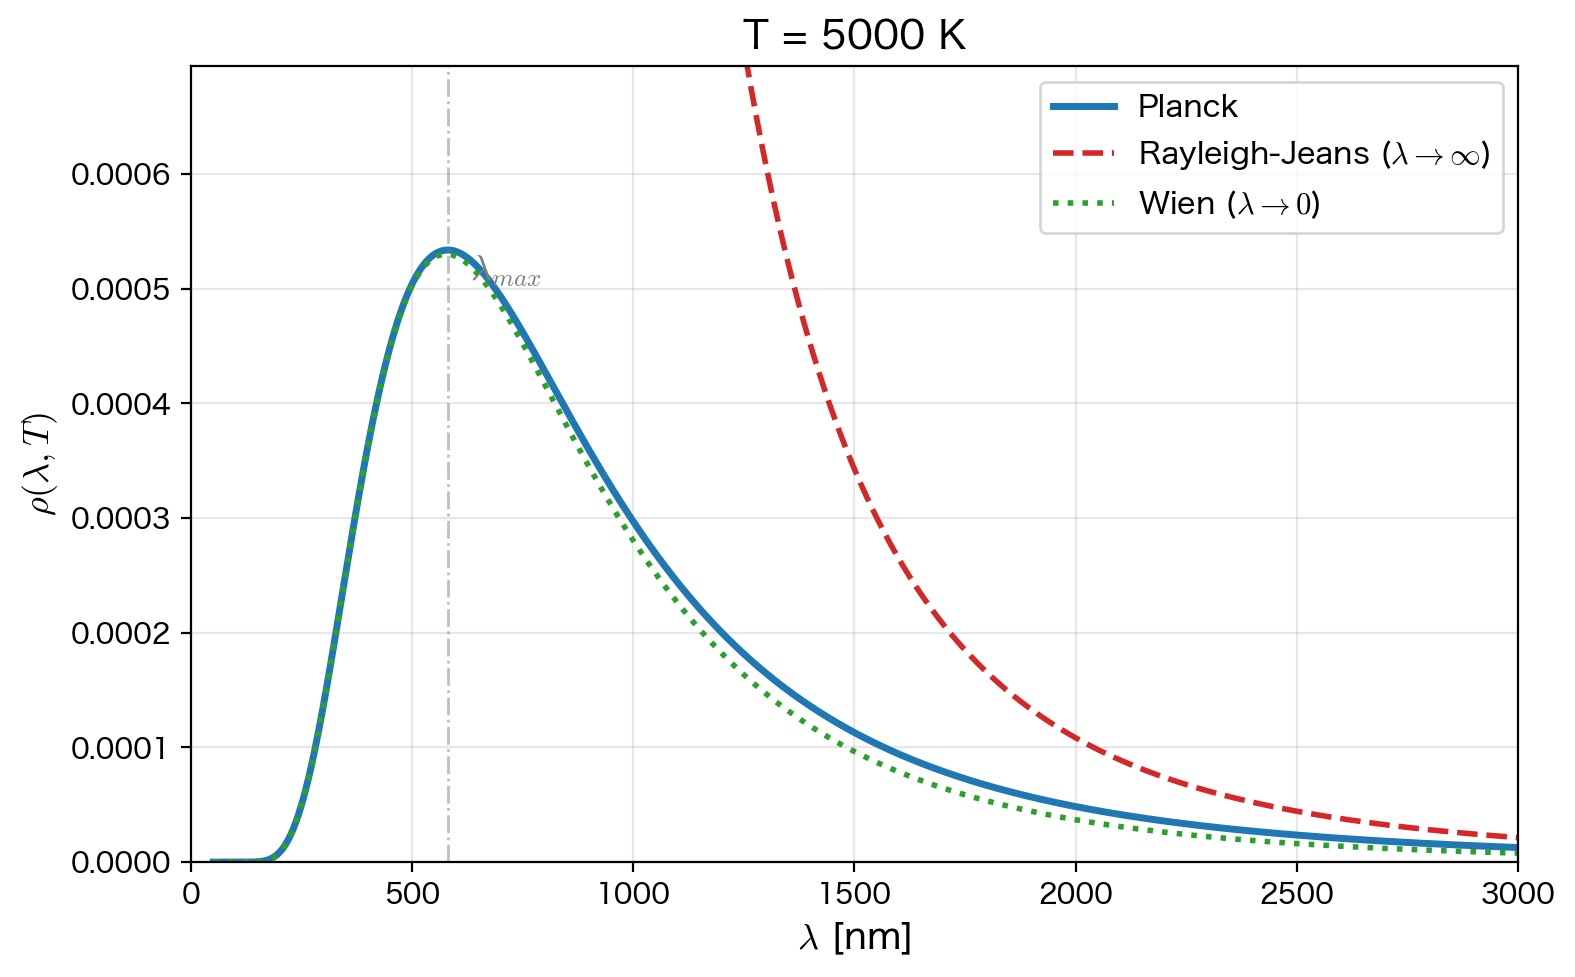
\includegraphics[width=0.95\textwidth]{figures/planck_with_limits.png}
\end{column}
\begin{column}{0.55\textwidth}
$\displaystyle\rho = \frac{8\pi hc}{\lambda^5}\frac{1}{e^{hc/\lambda k_\text{B}T} - 1}$

\vspace{0.3em}
\textbf{短波長}（$\lambda \to 0$）：$\rho \to 0$（Wien分布）

\vspace{0.2em}
\textbf{長波長}（$\lambda \to \infty$）：$e^x \approx 1+x$より
\[
  \rho \approx \frac{8\pi k_\text{B}T}{\lambda^4} \quad \text{（Rayleigh-Jeans）}
\]
\end{column}
\end{columns}
\end{frame}

% ============================================================
\begin{frame}[shrink=5]{Wien の法則とStefan-Boltzmann の法則}

\textbf{① Wienの変位則：}$\rho$が最大となる波長$\lambda_\text{max}$
\[
  \frac{d\rho}{d\lambda}\bigg|_{\lambda=\lambda_\text{max}} = 0
  \quad \Longrightarrow \quad
  \lambda_\text{max}T = \text{const}
\]

\teacher{$T$が高いほど$\lambda_\text{max}$は短波長に移動する。\\
太陽（$\sim\SI{5800}{K}$）の放射ピークが可視光域にあるのはこのため。}

\vspace{0.3em}
\textbf{② Stefan-Boltzmannの法則：}全放射エネルギー密度$U$
\[
  U = \int_0^\infty \rho(\lambda,T)\,d\lambda \propto T^4
\]

導出のポイント：$x = hc/(\lambda k_\text{B}T)$と置換し，
$\displaystyle\int_0^\infty \frac{x^3}{e^x - 1}dx = \frac{\pi^4}{15}$を使う。

\importantbox{
  $U = \dfrac{8\pi^5 k_\text{B}^4}{15h^3c^3}\,T^4 \propto T^4$
}
\end{frame}

% %%%%%%%%%%%%%%%%%%%%%%%%%%%%%%%%%%%%%%%%%%%%%%%%%%%%%%%%%%%%
\section{まとめ}
% %%%%%%%%%%%%%%%%%%%%%%%%%%%%%%%%%%%%%%%%%%%%%%%%%%%%%%%%%%%%

% ============================================================
\begin{frame}[shrink=5]{全体のまとめ}

\begin{enumerate}
  \item \textbf{量子論の誕生}\\
    Planck → Einstein → de Broglie → Schrödinger

  \item \textbf{井戸型ポテンシャル}\\
    $\psi_n = \sqrt{2/a}\sin(n\pi x/a)$，\;$E_n = n^2 h^2/(8ma^2)$

  \item \textbf{物理的意味}\\
    $|\psi|^2$＝確率密度，零点エネルギー，対応原理

  \item \textbf{調和振動子}\\
    $E_n = (n+\frac{1}{2})\hbar\omega$，赤外吸収，Morseポテンシャル

  \item \textbf{黒体放射の定量}\\
    Planck分布の極限，Wien則，Stefan-Boltzmann則
\end{enumerate}
\end{frame}

% ============================================================
\begin{frame}[shrink=5]{入試対策チェックリスト}

\begin{block}{これができれば合格ラインです：}
  {\small
  \begin{tabular}{cl}
    $\square$ & 変数分離 → 境界条件 → 規格化（半角公式）の再現 \\
    $\square$ & 零点エネルギーを不確定性原理で説明 \\
    $\square$ & 共役ポリエンの吸収波長$\lambda$の計算 \\
    $\square$ & 調和振動子の$E_n$，換算質量，振動波数 \\
    $\square$ & Morse vs 調和振動子の違いを図示 \\
    $\square$ & Planck分布の長波長/短波長極限の導出 \\
    $\square$ & Wien則・Stefan-Boltzmann則の導出 \\
  \end{tabular}
  }
\end{block}
\end{frame}

% ============================================================
\begin{frame}[standout]
  頑張れ！
\end{frame}

\end{document}
